\documentclass[a4paper, margin=1in]{article}
%\usepackage{CJK}
\usepackage{latexsym}
\usepackage{color}
\usepackage[x11names]{xcolor} % for a set of predefined color names, like LemonChiffon1
\usepackage{graphicx, float}\usepackage{graphicx}
\usepackage{algorithmic}
\usepackage{algorithm}
%\usepackage{algpseudocode}
%\usepackage[colorlinks]{hyperref}
\usepackage[toc,page]{appendix}
\usepackage{bm}
\setlength{\oddsidemargin}{-0.0in}
\setlength{\evensidemargin}{-0.0in} \setlength{\textwidth}{6.0in}
\setlength{\textheight}{9.0in} \setlength{\topmargin}{-0.2in}
%\usepackage[boxruled]{algorithm2e}

%\setlength{\leftmargin}{0.7in}
\usepackage{amssymb, graphicx, amsmath}  %  fancyheadings,
\usepackage{setspace}
\newcommand\qed{\qquad $\square$}
\newcommand{\nn}{\nonumber}

\usepackage{lipsum}

\usepackage{listings}
\lstset{
  basicstyle=\ttfamily,
  columns=fullflexible,
  frameround=fttt,
  breaklines=true,
  %postbreak=\mbox{\textcolor{red}{$\hookrightarrow$}\space},
}

\definecolor{mGreen}{rgb}{0,0.6,0}
\definecolor{mGray}{rgb}{0.5,0.5,0.5}
\definecolor{mPurple}{rgb}{0.58,0,0.82}
\definecolor{backgroundColour}{rgb}{0.95,0.95,0.92}

\lstdefinestyle{CStyle}{
basicstyle=\ttfamily,
language=C,
numberstyle=\tiny\color{mGray},
numbers=left,
frame=lines,
framexleftmargin=0.5em,
framexrightmargin=0.5em,
backgroundcolor=\color{LemonChiffon1},
showstringspaces=false,
escapeinside={(*@}{@*)},
}

\def \[{\begin{equation}}
\def \]{\end{equation}}
\def\proof{{\bf Proof:\quad}}
\def \endzm {\quad $\Box$}
\def\dist{\hbox{dist}}

\usepackage{tabularx,booktabs}
\newcolumntype{C}{>{\centering\arraybackslash\hsize=.5\hsize}X} % centered version of "X" type
\setlength{\extrarowheight}{1pt}
\usepackage{caption}% <-- added


\newcommand{\R}{\mathbb{R}}
%\newtheorem{yinli}{����}[section]
\newcommand{\D}{\displaystyle}
\newcommand{\T}{\textstyle}
\newcommand{\SC}{\scriptstyle}
\newcommand{\FT}{\footnotesize}

\usepackage{hyperref}
\newcommand\fnurl[2]{%
  \href{#2}{#1}\footnote{\url{#2}}%
}


%\newtheorem{theorem}{Theorem}[section]
%\renewcommand{\thetheorem}{\arabic{section}.\arabic{theorem}}
\newtheorem{definition}{Definition}
\renewcommand{\thedefinition}{\arabic{section}.\arabic{definition}}
\newtheorem{lemma}{Lemma}[section]
\renewcommand{\thelemma}{\arabic{section}.\arabic{lemma}}
\newtheorem{remark}{Remark}
\renewcommand{\theremark}{\arabic{section}.\arabic{remark}}
\newtheorem{proposition}{Proposition}[section]
\renewcommand{\theproposition}{\arabic{section}.\arabic{proposition}}
\newtheorem{corollary}{Corollary }[section]
\renewcommand{\thecorollary}{\arabic{section}.\arabic{corollary}}
\renewcommand{\theequation}{\arabic{section}.\arabic{equation}}
\renewcommand{\baselinestretch}{1.35}
\newtheorem{exam}{Example}[section]
\renewcommand{\theexam}{\arabic{section}.\arabic{exam}}
\newtheorem{theo}{Theorem}[section]
\renewcommand{\thetheo}{\arabic{section}.\arabic{theo}}

% Define a \HEADER{Title} ... \ENDHEADER block
\makeatletter
\newcommand{\HEADER}[1]{\ALC@it\underline{\textsc{#1}}\begin{ALC@g}}
\newcommand{\ENDHEADER}{\end{ALC@g}}
\makeatother

\newcommand{\argmin}{\operatornamewithlimits{argmin}}
\newcommand{\argmax}{\operatornamewithlimits{argmax}}

\usepackage{url} % to make url in bibtex shows up

% Create a command to cleanly insert a snippet with the style above anywhere in the document
\newcommand{\insertcode}[2]{\begin{itemize}\item[]\lstinputlisting[caption=#2,label=#1,style=CStyle]{#1}\end{itemize}} % The first argument is the script location/filename and the second is a caption for the listing

\begin{document}
%\begin{CJK*}{GBK}{song}

\begin{center}

{\LARGE \bf CS380L: Advanced Operating Systems Lab \#1}\\

\vskip 25pt
 {Zeyuan Hu \footnote{30 hours spent on this lab.}, iamzeyuanhu@utexas.edu }\\
\vskip 5pt
{\small EID:zh4378 Spring 2019 }

\end{center}

\begin{spacing}{1.5}
\section{Environment} \label{environment}

We use a Linux server for all the experiments. The server has 4 Intel(R) Xeon(R) CPU E3-1220 v5 @ 3.00GHz processors and 16GB of memory, and runs Ubuntu 16.04.2 LTS (kernel version 4.11.0). The CPU has 32KB of L1 data cache per core (8-way set associative) (found through \lstinline!getconf -a | grep CACHE!). In addition, it has two-level TLBs. The first level (data TLB) has 64 entries (4-way set associative), and the second level has 1536 entries for both instructions and data (6-way set associative) (found through \lstinline!cpuid | grep -i tlb!).

\section{Memory map}

\lstinline|/proc/[pid]/maps| file contains process \lstinline|[pid]|'s mapped memory regions and their access permissions \cite{proc_man}. We use
the following code to read content of \lstinline|/proc/self/maps| file \footnote{see \texttt{memory\_map.c} for complete code}:

%\insertcode{"../src/memory_map.c"}{Code for memory map task}
\begin{lstlisting}[style=CStyle]
sprintf(filepath, "/proc/%u/maps", (unsigned)getpid());
FILE *f = fopen(filepath, "r");

printf("%-32s %-8s %-10s %-8s %-10s %s\n", "address", "perms", "offset", "dev", "inode", "pathname");
while (fgets(line, sizeof(line), f) != NULL) {
     sscanf(line, "%s%s%s%s%s%s", address, perms, offset, dev, inode, pathname);
     printf("%-32s %-8s %-10s %-8s %-10s %s\n", address, perms, offset, dev, inode, pathname);
}
fclose(f);
\end{lstlisting}

In the file, each line corresponds to a mapped memory region. There are six columns of each line, which represent six properties of the mapped memory region: \texttt{address}, \texttt{perms}, \texttt{offset}, \texttt{dev}, \texttt{inode}, and \texttt{pathname}. The result of running \texttt{memory\_map.c} is below:

\begin{figure}
	\centering
	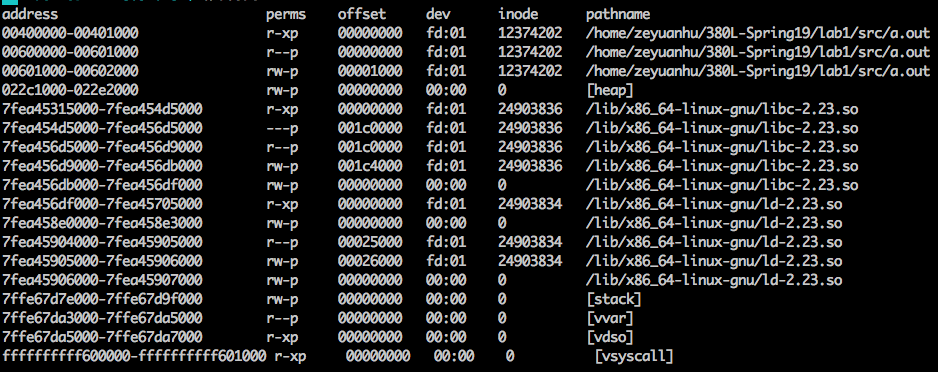
\includegraphics[scale=0.5]{memory_map.png} 
	\caption{Output of memory\_map.c}
	\label{memory_map}
\end{figure}

The \texttt{address} field gives range of virtual memory address of the mapped memory region. Access permission of each memory region is indicated by \texttt{perms} field. 
There are four bits in the field: \texttt{rwx} represents read, write, and executable respectively; the last bit (\texttt{p} or \texttt{s}) represents whether the region is private or shared. \texttt{offset} field represents the offset in the mapped file. \texttt{dev} field indicates the device (represented with format of \texttt{major:minor}) that the mapped file resides . There are two kinds of value in this column for our case: \texttt{fd:01} and \texttt{00:00}. The former one is the device id (in hex) of \texttt{/} (checked with \lstinline|mountpoint -d /|) and the latter one represents no device associated with the file.
\texttt{inode} field represents the inode number of the file on the device. \texttt{0} means no file is associated with the mapped memory region. \texttt{pathname} field gives the absolute path to the file associated with the mapped memory region. It can be some special values like \texttt{[heap]}, \texttt{[stack]}, \texttt{[vdso]}, etc.

To locate the start of the text section of the executable, we invoke \texttt{objdump -h} on the binary and get \texttt{0000000000400600}.  Output of \texttt{/proc/self/maps} shows that the start address of \texttt{libc} is \texttt{7fea45315000}. The reason for these two addresses are different is \texttt{libc} is dynamic loaded library, which is loaded during the runtime of executable, which is not compiled and linked as part of executable. The code segment contains the executable instruction, not the dynamic loaded library.

One interesting thing happens between runs of the executable: the content of \texttt{/proc/self/maps} is different. Addresses of all mapped memory regions are different except for the regions mapped to the executable and \texttt{[vsyscall]}. The root cause behind this phenomenon is Address Space Layout Randomization (ASLR) \cite{aslr} for programs in user space. This feature is enabled by default and can be seen via the content of \lstinline|/proc/sys/kernel/randomize_va_space| file. In our case, the value is 2, which means the positions of stack itself, virtual dynamic shared object (VDSO) page, shared memory regions, and data segments are randomized \cite{aslr2}.

\section{Getrusage}

To get resource usage of the current process, we use \texttt{getrusage} \cite{getrusage_man}. The result is stored in \texttt{rusage} struct. Not all fields of the struct
are completed: unmaintained fields are set to zero by the kernel. Those fields exist for compatibility with other systems purpose. The following code instantiates \texttt{rusage} struct and print all the maintained fields \footnote{complete code can be seen in \texttt{getrusage.c}}:

\begin{lstlisting}[style=CStyle]
struct rusage usage;
if (getrusage(RUSAGE_SELF, &usage) != 0) {
    perror("getrusage");
    return 0;
}

// user CPU time used
printf("utime = %ld.%06ld s\n", usage.ru_utime.tv_sec,
usage.ru_utime.tv_usec);
// system CPU time used
printf("stime = %ld.%06ld s\n", usage.ru_stime.tv_sec,
usage.ru_stime.tv_usec);
// maximum resident set size
printf("maxrss = %ld KB\n", usage.ru_maxrss);
// page reclaims (soft page faults)
printf("minflt = %ld\n", usage.ru_minflt);
// page faults (hard page faults)
printf("majflt = %ld\n", usage.ru_majflt);
// block input operations
printf("inblock = %ld\n", usage.ru_inblock);
// block output operations
printf("oublock = %ld\n", usage.ru_oublock);
// voluntary context switches
printf("nvcsw = %ld\n", usage.ru_nvcsw);
// involuntary context switches
printf("nivcsw = %ld\n", usage.ru_nivcsw);
\end{lstlisting}

man page of \texttt{getrusage} explains the meaning of each field \cite{getrusage_man} in details. \texttt{utime} and \texttt{stime} are about CPU time usage; \texttt{minflt} and \texttt{majflt} are related to page faults; \texttt{maxrss} represents the maximum size of working set; \texttt{inblock} and \texttt{oublock} are about file system I/O. 

\section{perf\_event\_open} 

We use the machine specified in the \ref{environment}, which is a physical server (i.e., not VM). We first check the support of \lstinline|perf_event_open| interface by checking the existence of \lstinline|/proc/sys/kernel/perf_event_paranoid|, which is true in our case (value is set to \texttt{2}). In Linux, \lstinline|perf_event_open| interface \cite{perf_event_open_man} is used to setup performance monitoring. Specifically, it provides an interface that allows user to access 
various events (i.e., events counted by performance counters \cite{hardware_counter}). \lstinline|perf list| gives available events on current machine. Counters related to cache in our machine is shown in Figure \ref{counters}. We are interested in counters related to L1 data cache and data TLB. As shown in Figure \ref{counters}, we have counters for number of times the L1 cache was accessed for data (\texttt{L1-dcache-loads}), the number of those access that resulted in a cache miss (\texttt{L1-dcache-load-misses}), and write access of L1 data cache (\texttt{L1-dcache-stores}). Similarly, for data TLB, we have read access (\lstinline|dTLB-loads|), read miss (\lstinline|dTLB-load-misses|), write access (\lstinline|dTLB-stores|), and write miss (\lstinline|dTLB-store-misses|).


\begin{figure}	
	\centering
	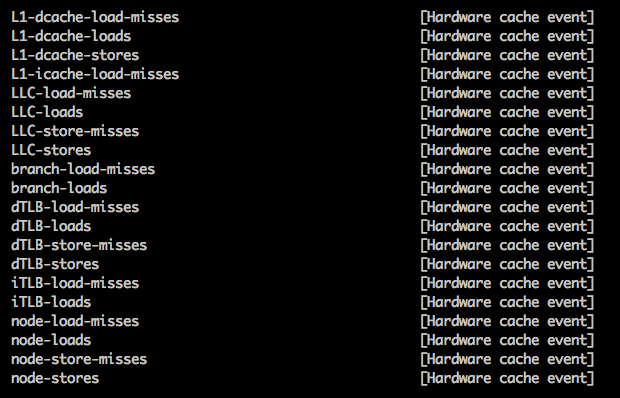
\includegraphics[scale=0.5]{counters.png} 
	\caption{Part of output of \texttt{perf list} related to cache}
	\label{counters}
\end{figure}


\end{spacing}
\bibliographystyle{ieeetr}
\bibliography{report}
\end{document}

